\begin{frame}{Observation: Identifying Patterns and Gaps}
  \begin{columns}
    \column{0.5\textwidth}
    \textbf{Processes:}
    \begin{itemize}
      \item Reviewing Scientific Literature
      \item Analysing Known Phenomena
      \item Examining Existing Data
      \item Identifying Unsolved Problems
    \end{itemize}

    \column{0.5\textwidth}
    \textbf{Results \& Connections:}
    \begin{itemize}
      \item Formulation of New Hypotheses
      \item Refinement of Existing Questions
      \vspace{1.81cm}
    \end{itemize}
  \end{columns}
\end{frame}

\begin{frame}{Nature of Light}
  \vspace{0.5cm}
  \begin{columns}
    \column{0.5\textwidth}
    \textbf{Newton's Idea}
    \begin{figure}
      \centering
      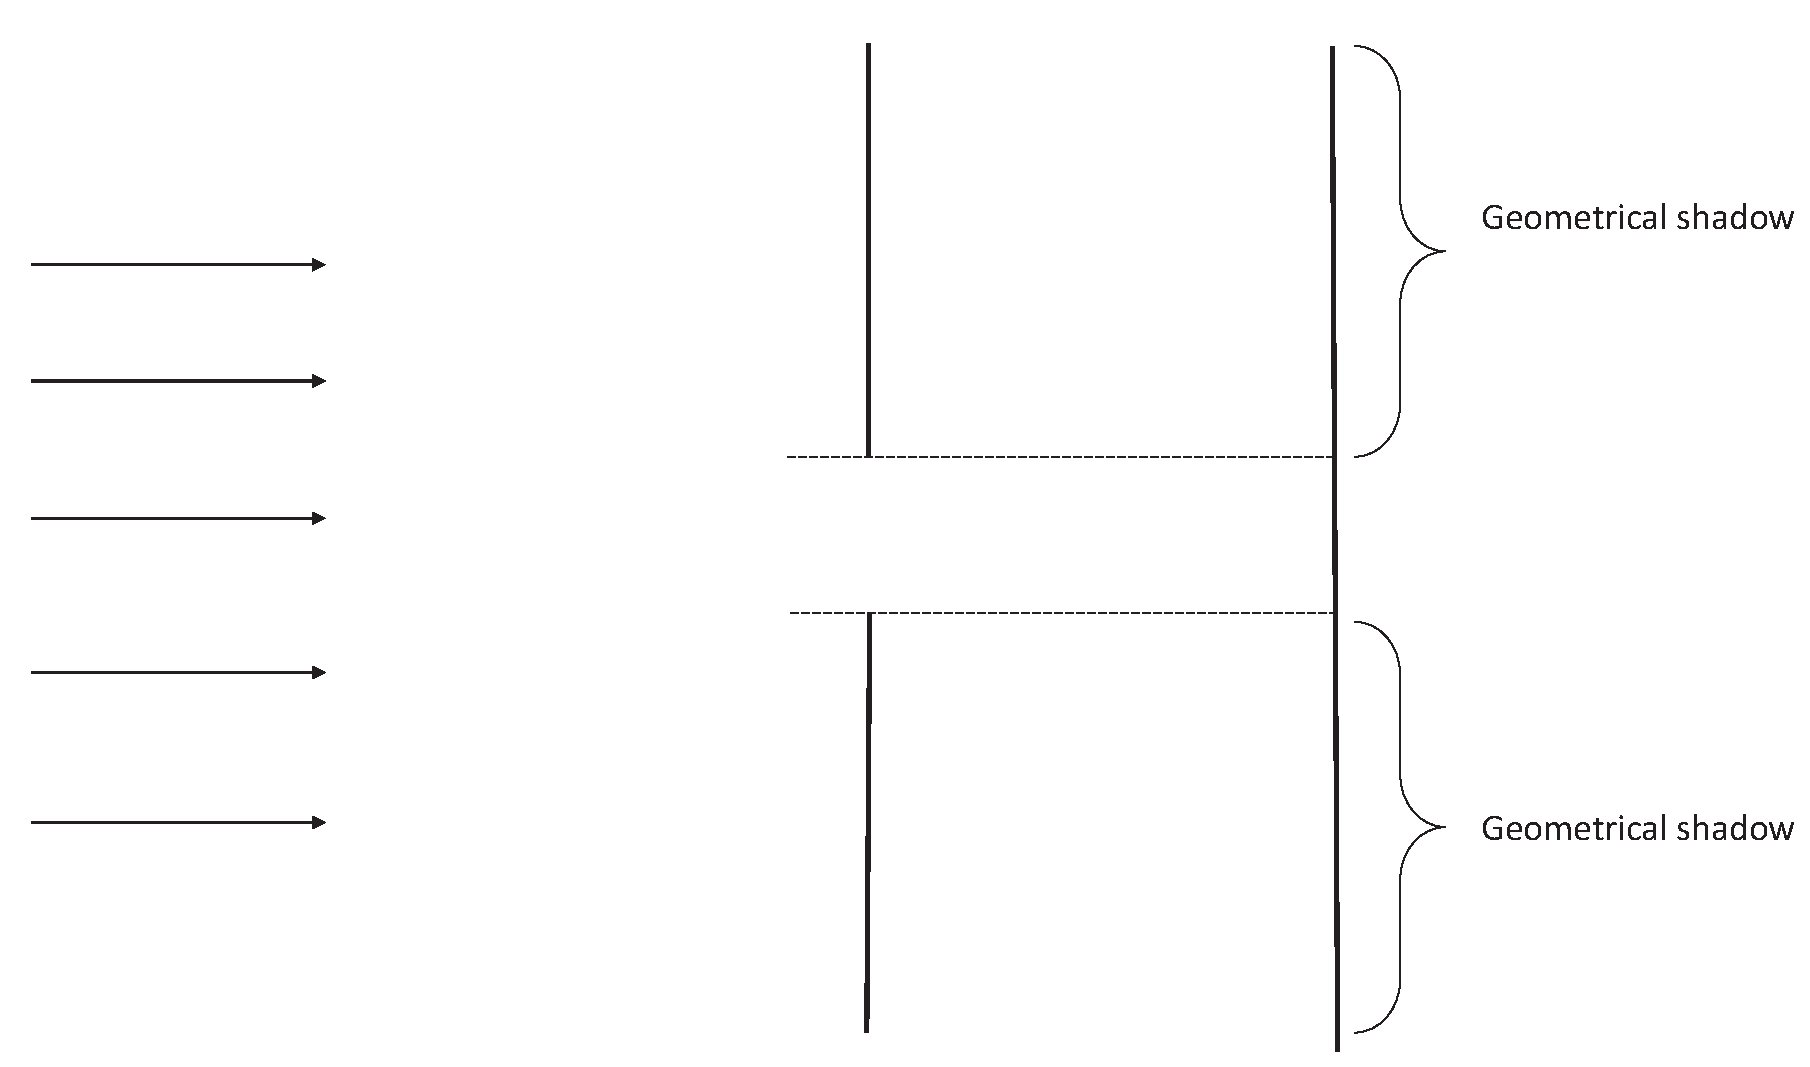
\includegraphics[width=\textwidth]{Figures/Fig1.pdf}
      \caption{Newton's particle theory of light.}
    \end{figure}

    \column{0.5\textwidth}
    \textbf{Huygens' Principle}
    \begin{figure}
      \centering
      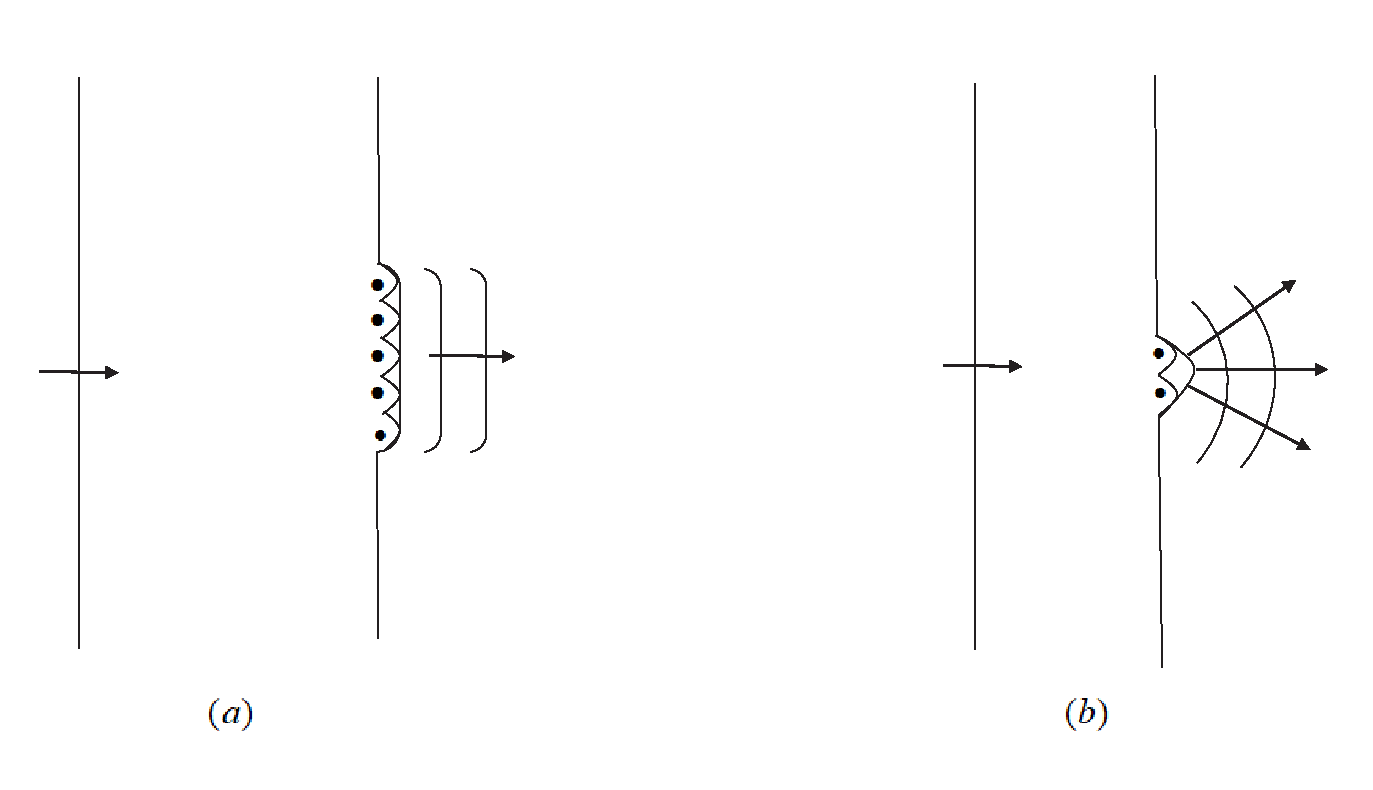
\includegraphics[width=\textwidth]{Figures/Fig5.pdf}
      \caption{Huygens' wave theory of light.}
    \end{figure}
  \end{columns}

  \vspace{0.5cm}
  \centering
  Observation showed that Newton was mistaken. \cite{Simeonov2024}
\end{frame}

\begin{frame}{Hypothesis Testing: Validating Scientific Claims}
  \begin{columns}
    \column{0.5\textwidth}
    \textbf{Processes:}
    \begin{itemize}
      \item Designing and Conducting Experiments
      \item Collecting and Analyzing Data
      \item Comparing Results with Predictions
    \end{itemize}

    \column{0.5\textwidth}
    \textbf{Results \& Connections:}
    \begin{itemize}
      \item Discovery of New Patterns or Anomalies
      \item Theory Development or Refinement
      \item Practical Applications in Technology or Industry
    \end{itemize}
  \end{columns}
\end{frame}

\begin{frame}{De Broglie hypothesis}
  \vspace{0.2cm}
  Louis De Broglie proposed that particles have associated waves. \cite{Broglie2021}

  \begin{figure}
    \centering
    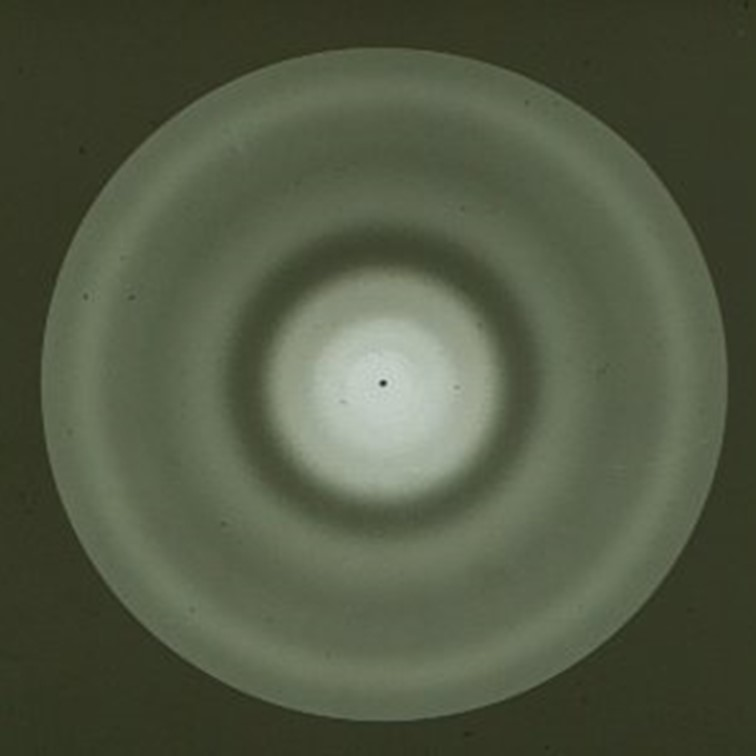
\includegraphics[width=0.5\textwidth]{Figures/electron-diffraction.jpg}
    \caption{Electron diffraction pattern—evidence of wave behaviour. \cite{NorbertMitzel2022}}
  \end{figure}
\end{frame}

\begin{frame}{Peer Feedback: Refining Scientific Knowledge}
  \begin{columns}
    \column{0.5\textwidth}
    \textbf{Processes:}
    \begin{itemize}
      \item Independent Replication of Experiments
      \item Peer Review and Critical Evaluation
      \item Scientific Discussions and Debates
      \item Integration into Theoretical Frameworks
    \end{itemize}

    \column{0.5\textwidth}
    \textbf{Results \& Connections:}
    \begin{itemize}
      \item Identification of Errors or Biases
      \item Generation of New Hypotheses
      \item Expansion of Scientific Applications
      \vspace{1.1cm}
    \end{itemize}
  \end{columns}
\end{frame}

\begin{frame}{Wave and particle or wave-particle behaviour}
  The Feedback from theories generated different interpretations. \cite{Struyve2001}

  \vspace{0.8cm}

  \begin{columns}
    \column{0.5\textwidth}
    \textbf{De Broglie-Bohm Theory}
    \begin{figure}
      \centering
      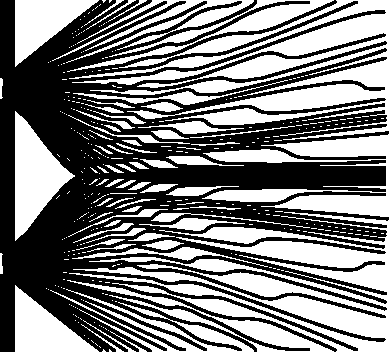
\includegraphics[width=0.9\textwidth]{Figures/doppel.pdf}
      \caption{Photon trajectories in the double slit experiment. \cite{Opasson2011}}
    \end{figure}
    
    \column{0.5\textwidth}
    \textbf{Copenhagen Interpretation}

    \vspace{0.8cm}

    \begin{equation*}
    \big| \psi(x, t) \big|^2
    \end{equation*}

    \vspace{1cm}
    Probabilistic interpretation of wavefunction collapse.
  \end{columns}
\end{frame}

\begin{frame}{Applications: Science in Action}
  \begin{columns}
    \column{0.5\textwidth}
    \textbf{Processes:}
    \begin{itemize}
      \item Development of New Technologies
      \item Implementation in Medicine, Engineering, and Society
      \item Identification of Emerging Challenges
    \end{itemize}

    \column{0.5\textwidth}
    \textbf{Results \& Connections:}
    \begin{itemize}
      \item New Observations for Future Research
      \item Inspiration for Novel Experimental Approaches
      \vspace{1.1cm}
    \end{itemize}
  \end{columns}
\end{frame}

\begin{frame}{Wave Nature in Analytical Techniques}
  Electron diffraction is used to determine crystal structures. \cite{Zhou2017}

  \vspace{0.2cm}

  \begin{figure}
    \centering
    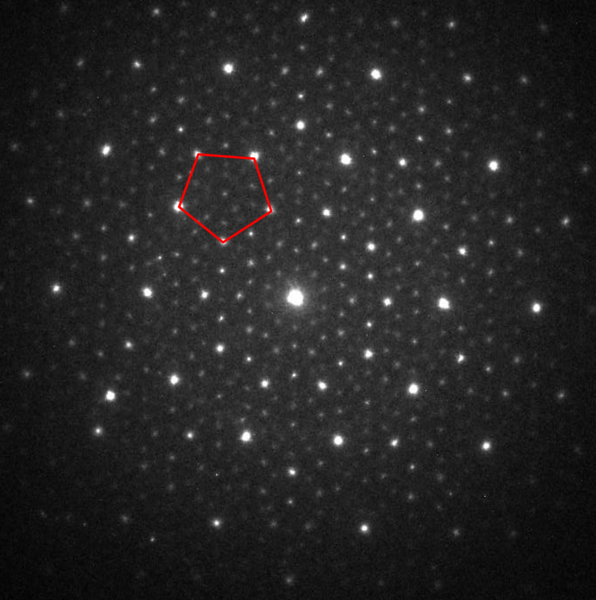
\includegraphics[width=0.5\textwidth]{Figures/crystal.png}
    \caption{Electron diffraction pattern of a decagonal quasicrystal of Al-Cu-Fe-Cr. \cite{Ldm19542003}}
  \end{figure}
  
\end{frame}
